\documentclass[12pt]{article}

\usepackage{amsmath}
\usepackage{amssymb}
\usepackage{geometry}
\usepackage{graphicx}
\usepackage{hyperref}

\geometry{letterpaper,tmargin=1in,bmargin=1in,lmargin=1in,rmargin=1in}

\hypersetup{
colorlinks, linkcolor=blue,
}


\begin{document}

\title{Analog Electronics}
\author{Laboratory exercise 5}
\date{Fall 2016}
\maketitle

\newpage
\section{Abstract}

In this experimentation we will be given the schematic of an Oscillating amplifier. With this and various equations, we will calculate the necessary value of $R_3$ using whatever capacitor we desire,to create a square wave oscillating at $500Hz$. Once we design this circuit we will then construct it ensuring that it operates as expected, and adjusting $R_3$ if necessary.

\section{Theory}
The model for this experimentation is the following figure.
\begin{figure}[h]
	\label{fig:amp}
	\caption{Given Amplifier}
	\centering
	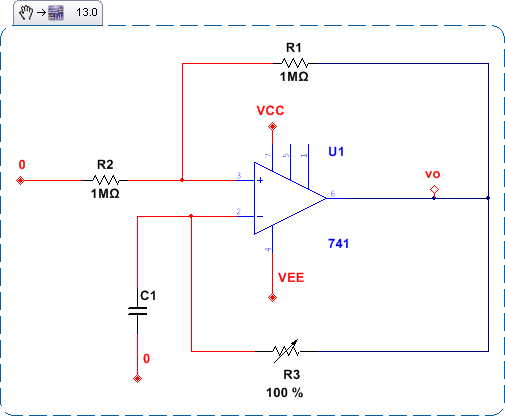
\includegraphics[width=1\textwidth]{opamp_oscillator}
\end{figure}

The following equation generates a square wave, where the time period of the square wave is given as:
$$ T = 2R_3C_1 \ln{\frac{1+\alpha}{1-\alpha}}, $$
\begin{center}
	 where $\alpha = \frac{R_2}{R_1 + R_2}$
\end{center}

By using the equation with a capacitor of our choosing we will have a equation with one unknown, $R_3$. Once we defined $R_3$ we can compare our calculated vs. our real-world measured values.

\section{Finding $R_3$}
To begin the process of find $R_3$ we must choose a capacitor value. The value that we will use in this experimentation is $C_1 = 1\mu F$. We will also be using the given values, $R_1=R_2=1M\Omega$\\

We begin by taking $500Hz$ and converting it to $T$ or time period. We can use the following equation
$$T = \frac{1}{Frequency}$$
$$T= \frac{1}{500Hz} = .002$$

Now we can solve for $\alpha$, with the given equation,
$$\alpha = \frac{R_2}{R_1 + R_2}$$
$$\alpha = \frac{1M\Omega}{1M\Omega+1M\Omega}$$
$$\alpha = 0.5M\Omega$$

Finally we can use the following equation to solve for $R_3$
$$ T = 2R_3C_1 \ln{\frac{1+\alpha}{1-\alpha}}, $$
$$.002=2R_3(1\mu F)ln(\frac{1+0.5}{1-0.5})$$
$$\frac{.002}{2}=R_3(1\mu F)ln(\frac{1+0.5}{1-0.5})$$
$$0.001=R_3(1\mu F)(1.098)$$
$$R_3 = \frac{0.001}{(1\mu F)(1.098)}$$
$$R_3 = 910.25$$

The value of $R_3$ that is needed to achieve a $500Hz$ square wave is $910.25\Omega$
\newpage
\section{Experimentation}
\subsection{Circuit Assembly}
 Gather the following devices for use in this experimentation.
	\begin{enumerate}
		\item 2 $1M\Omega$ Resistors
		\item $1K\Omega$ 1 turn potentiometer
		\item $741$ Operational Amplifier
		\item $1\mu F$ Capacitor
	\end{enumerate}
To set our potentiometer,
\begin{enumerate}
	\item Turn on the DMM and set it to ohmmeter mode.
	\item Measure between the middle pin and one of the outside pins on the potentiometer.(these will be the pins used in the experimentation)
	\item Turn the screw on the potentiometer until the DMM measures a value near our calculated $R_3=910\Omega$
\end{enumerate}
Construct the circuit as shown in Figure 1 ensuring that you use the same pins that where set on the potentiometer in the previous step.
\subsection{Testing}
We will now use the occiliscope to compare the waves at $V_O$ and across our capacitor $C_1$
\begin{enumerate}
	\item Begin first by powering on the occiliscope and connecting a probe to channel 1 and 2.
	\item Attach the channel 1 probe to our $V_0$, with the reference to ground.
	\item Attach the channel 2 probe across $C_1$.
	\item The "AUTOSET" function on the occiliscope provides presentation of both waveforms.
\end{enumerate}
\subsection{Achieving $500Hz$}
The data that occiliscope displayed showed that our desired $V_0$ frequency of $500Hz$ was not met. We can tweak our potentiometer to finalize our experimentation.
\\
By twisting our potentiometer screw we can vary our resistance enough to reach our final frequency of $500Hz$. Once you achieve this, power of the circuit, remove the potentiometer and measure the new $R_3$ value.

\newpage
\section{Comparing Waveforms}
The following image is of the occiliscope and the waveforms that were created with the oscillating amplifier with our new $R_3$ value of $798.7\Omega$.
\begin{figure}[!h]
	\label{fig:amp}
	\caption{$V_O$ compared to $C_1$}
	\centering
	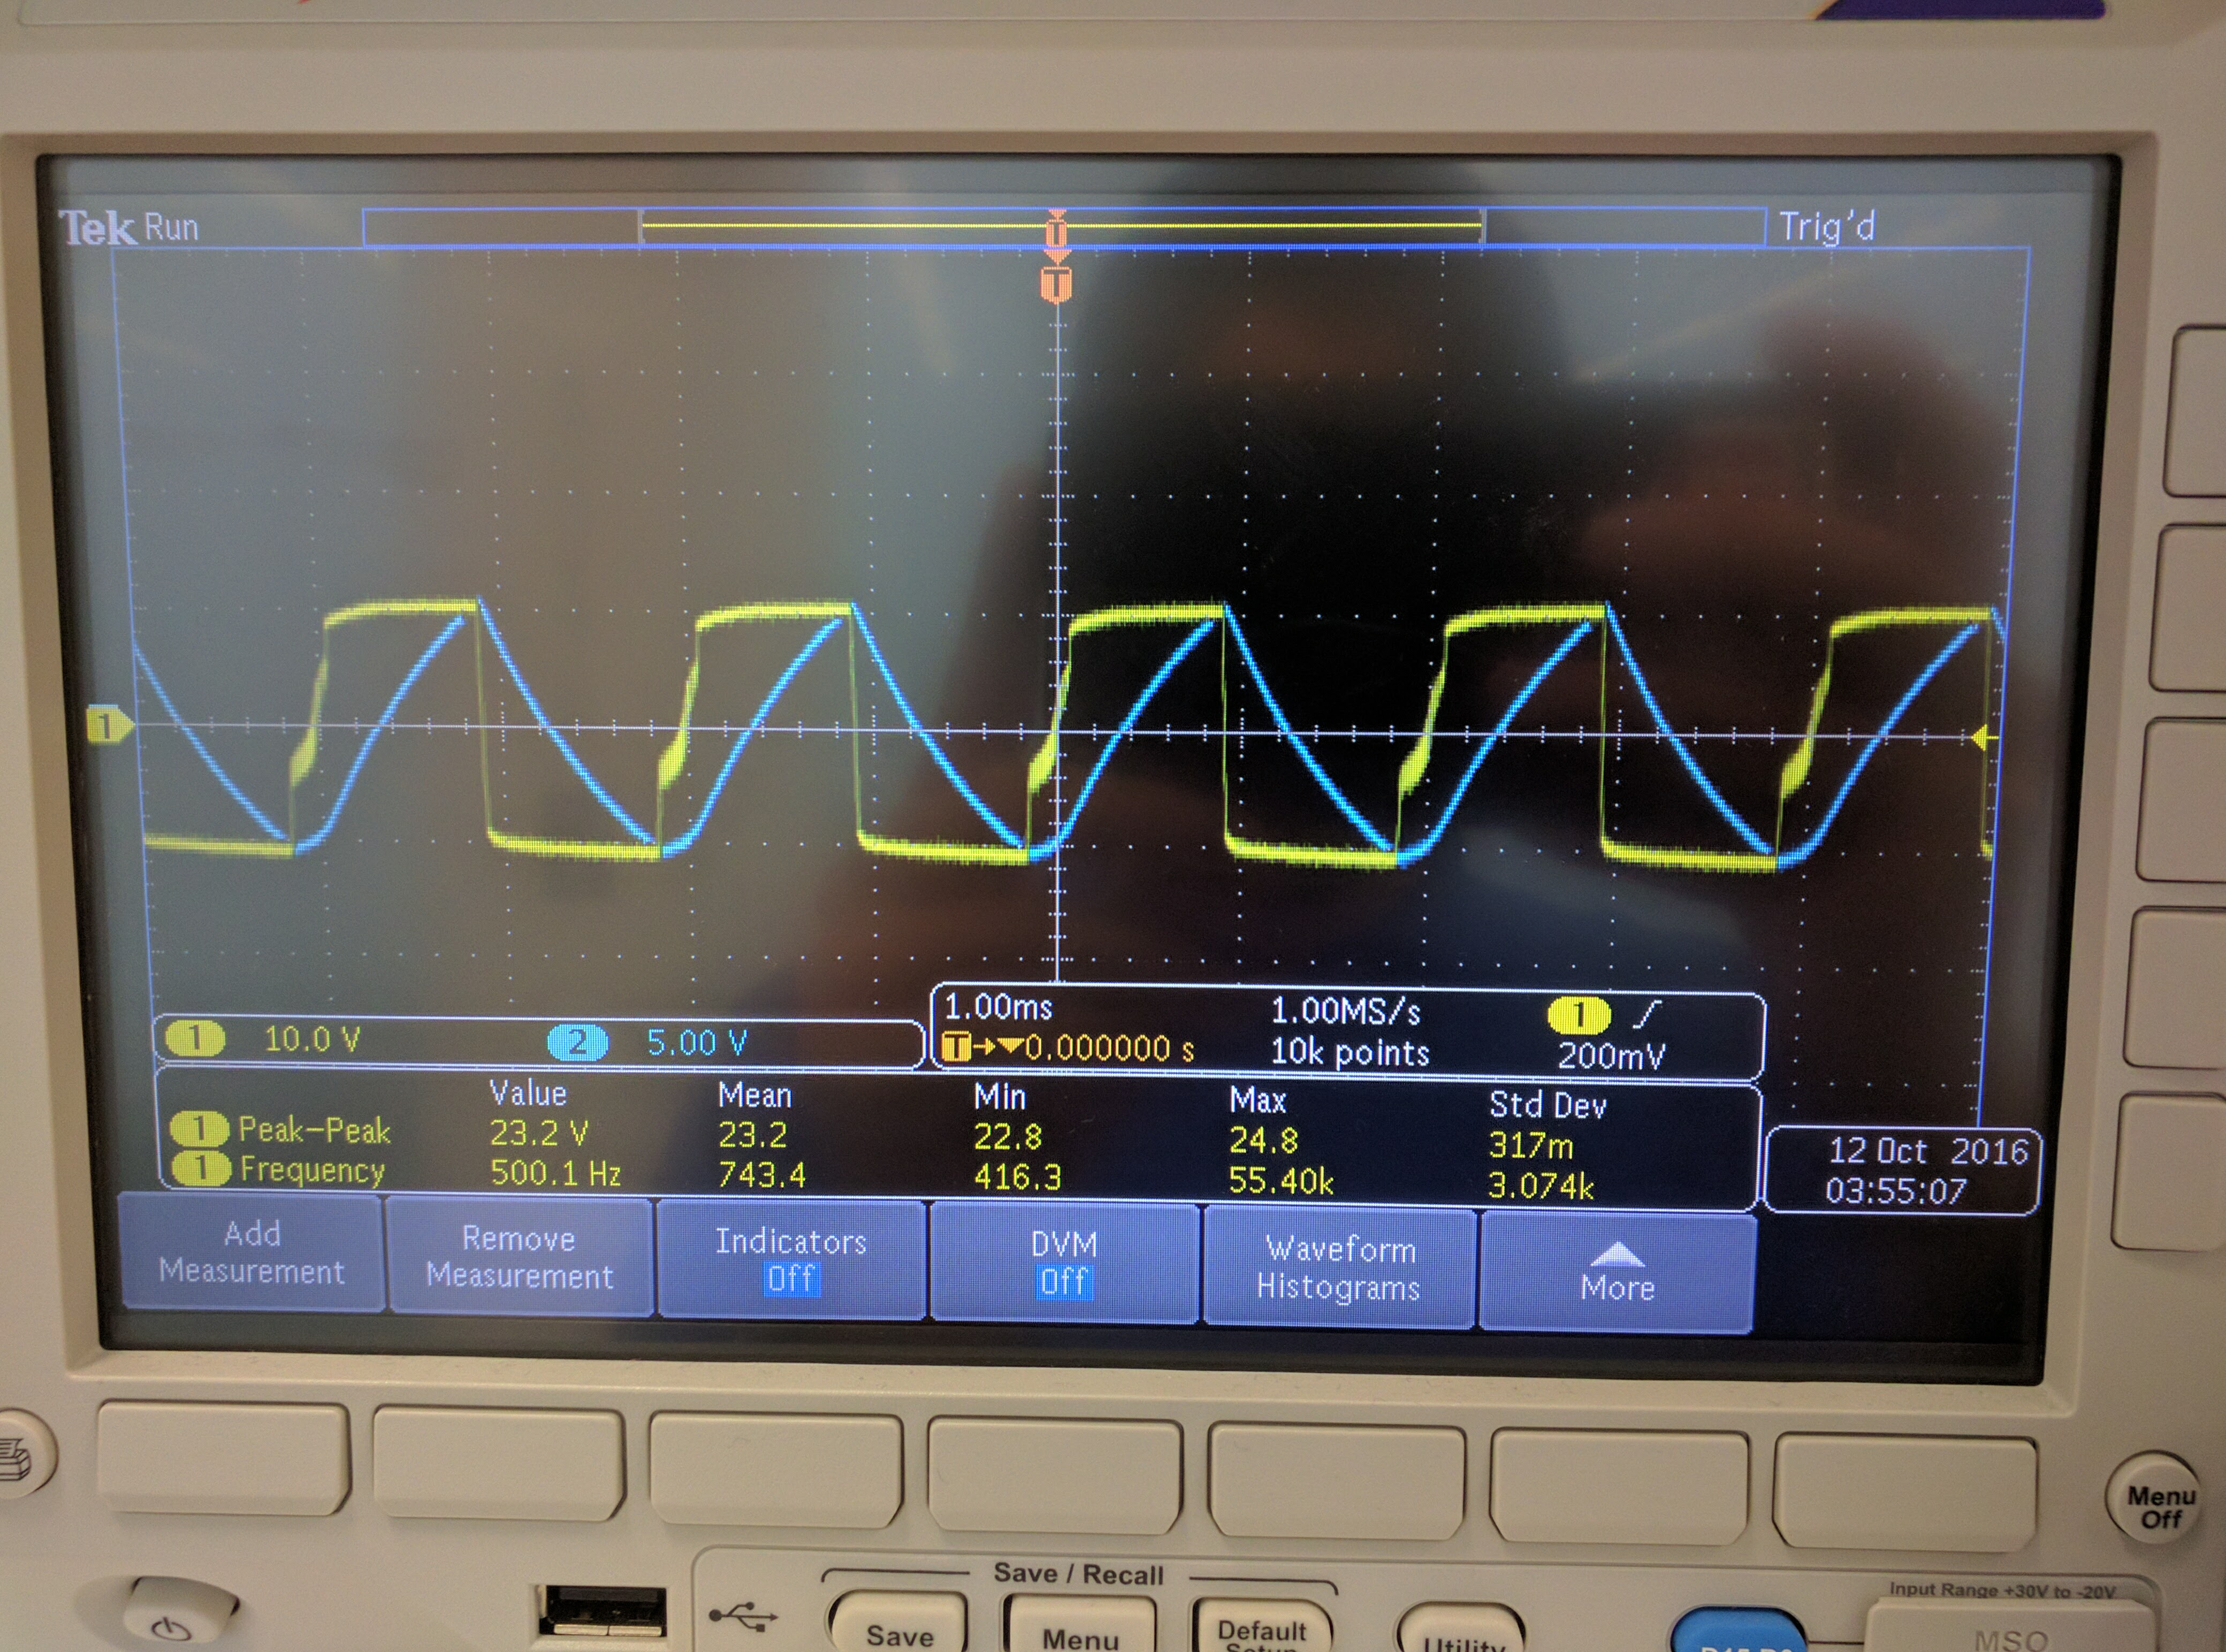
\includegraphics[width=1\textwidth]{waveform}
\end{figure}


\section{Conclusion}

In this experimentation we used a variety of analysis techniques to calculate and design an amplifier that took a DC voltage and created a square waveform from it. The experimentation allowed us to visualized simulated vs. real-world values. During that we also derived a $R_3$ value that we then manipulated to get us our desired frequency. One problem that occurred in this experimentation was an odd artifact on the $V_O$ square wave. It was later discovered a greater resistance value in combination with a smaller capacitor would've helped to remove the a deformity. Overall the experiment was yet another example of the usefulness of the 741 operational amplifier.

\end{document}